\documentclass[a4paper, 12pt, margins=2.5cm]{homework}
\usepackage{tikz}

\usepackage{graphicx}
\usepackage{dsfont}
\usepackage{microtype}
\usepackage{mathrsfs}
\usepackage[ngerman]{babel}
\usepackage{csquotes}
\usepackage[T1]{fontenc}
\usepackage{lmodern}
\usepackage{wasysym}

\setlength{\parindent}{0pt}

\newcommand{\R}{\mathbb{R}}
\newcommand{\N}{\mathbb{N}}
\newcommand{\Z}{\mathbb{Z}}
\newcommand{\Q}{\mathbb{Q}}
\newcommand{\C}{\mathbb{C}}

\name{Tobias Eidelpes}
\course{Objektorientierte Modellierung}
\term{2016SS}
\hwnum{5}
\hwtype{Übungsblatt}
\problemtitle{Aufgabe}
\solutiontitle{Lösung}

\begin{document}
  

  \problemnumber{1}
  \begin{problem}
    
  \end{problem}
  \begin{solution}\hfill
    \begin{center}
      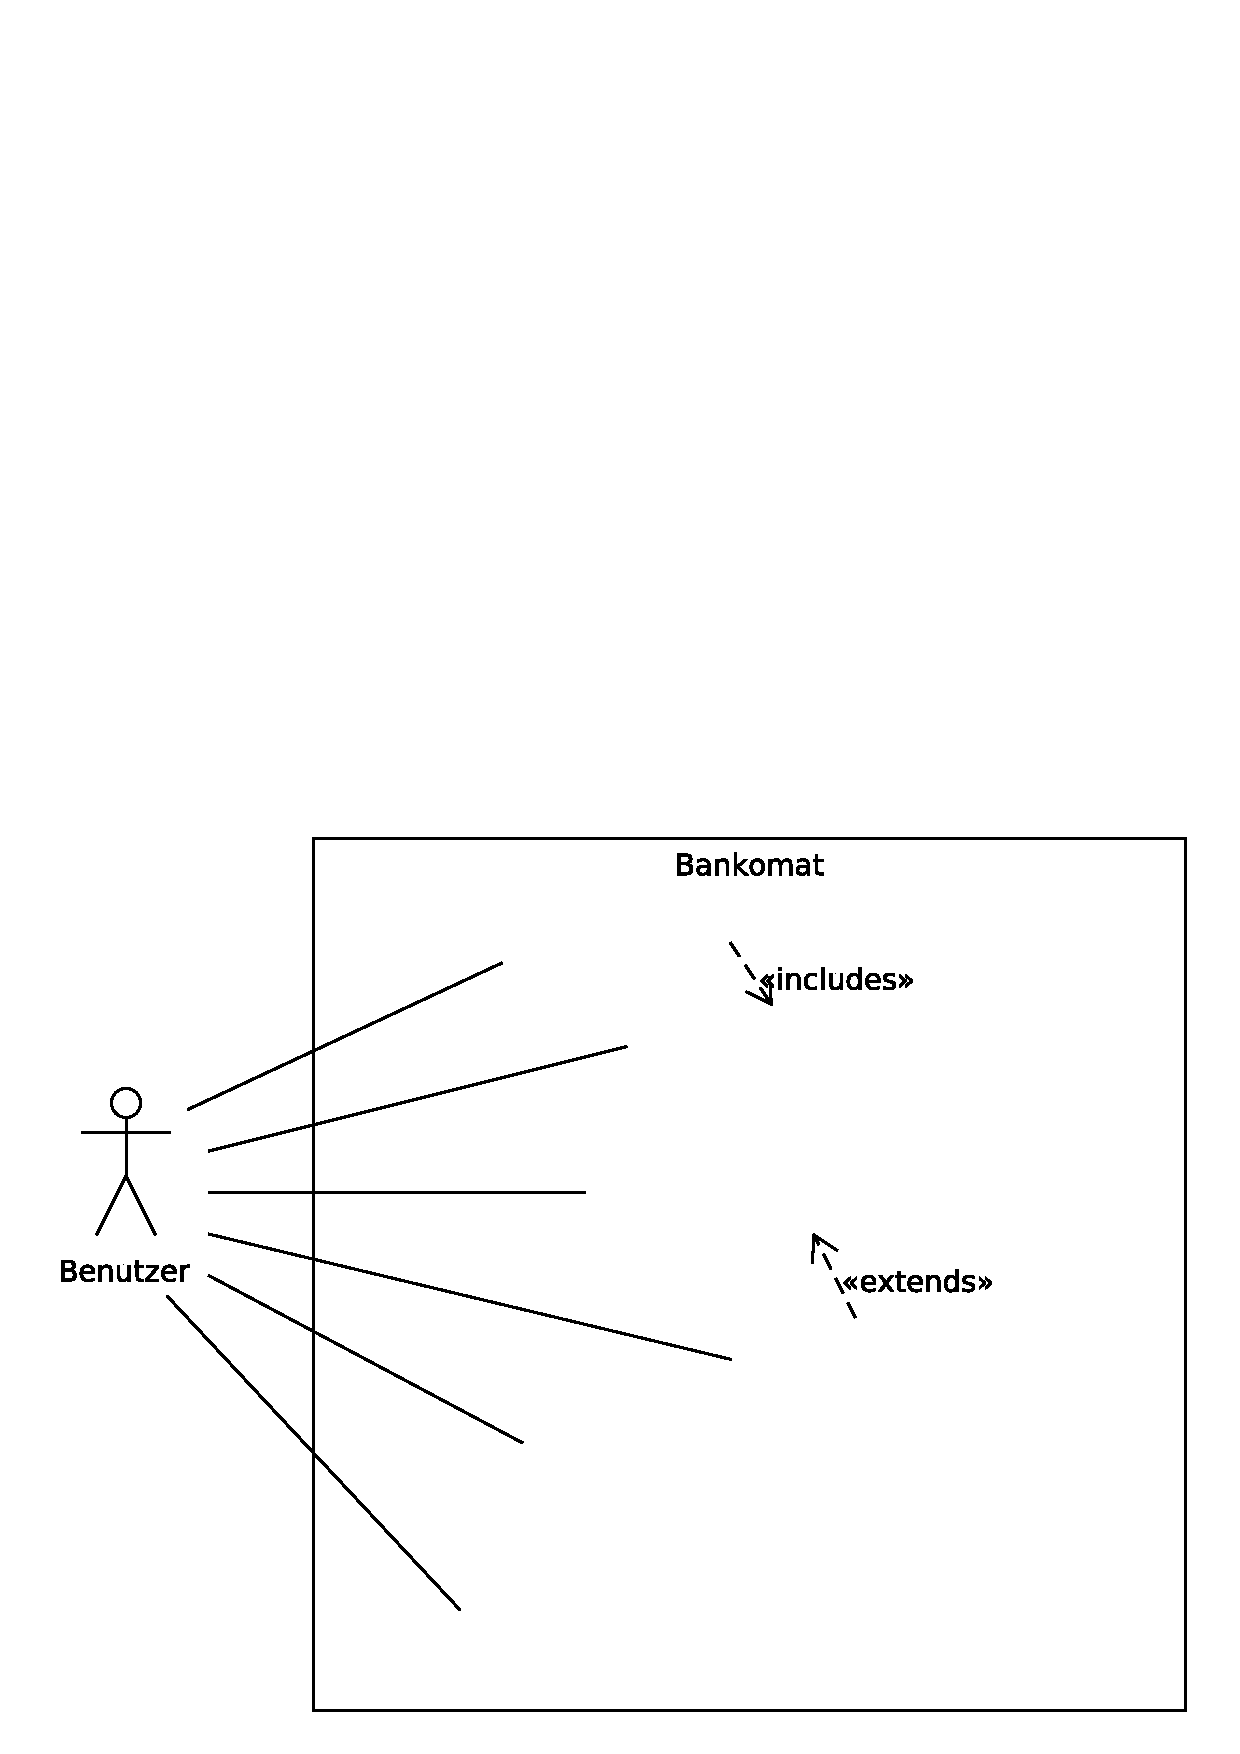
\includegraphics[scale=0.6]{Theoriebsp.pdf}
    \end{center}
    \begin{enumerate}[label=\alph*)]\itemsep0pt
      \item In diesem Beispiel haben wir einen Akteur, den Benutzer, welcher mit
            dem System Bankomat interagiert. Die Interaktion umfasst nun mehrere
            Möglichkeiten. Der Benutzer kann die Karte einführen, seinen Pincode
            eingeben, die gewünschte Summe eingeben, die Banknoten auswählen, seine
            Karte entnehmen und das Geld entnehmen. Das sind alles Use-Cases. Außerdem
            gibt es noch Beziehungen zwischen den einzelnen Anwendungsfällen: die
            \emph{include}- und die \emph{extend}-Beziehung. In diesem Beispiel
            leider nicht vorhanden sind Generalisierungen.

      \item Anwendungsfälle stellen alle möglichen Fälle dar, wie ein Benutzer ein
            System nutzen kann. Quasi die Anforderungen des Kunden an ein System.

      \item 

      \item Akteure sind ja Nutzer des Systems oder werden vom System benutzt. 
            Daher sind Akteure diejenigen die mit dem System interagieren.
            Anwendungsfälle sind Möglichkeiten, wie ein Akteur mit dem System
            interagieren kann.
    \end{enumerate}
  \end{solution}
  
  
  \problemnumber{2}
  \begin{problem}
    
  \end{problem}
  \begin{solution}\hfill
    \begin{enumerate}[label=\alph*)]\itemsep0pt
      \item Es gibt einerseits Akteure, die ein System benutzen und andererseits
            Akteure die vom System benutzt werden. Akteure repräsentieren überdies
            Rollen des Benutzers. Weiters können Akteure als menschlich und
            nicht-menschlich klassifiziert werden. Sowie als primär oder sekundär
            und aktiv oder passiv.
            Nicht-menschliche sekundäre und passive Akteure werden eher als Rechteck
            mit einem <<actor>> dargestellt. Menschliche primäre und aktive Akteure
            als Strichmanderl.

      \item Sowohl Akteure als auch Anwendungsfälle können generalisiert werden.
            Zum Beispiel kann ich mehrere Use-Cases, die irgendwie zusammengehören
            mithilfe von Generalisierungen zusammenfassen. Bei Akteuren kann ich
            zum Beispiel verschiedene Mitarbeiter unter dem Begriff Mitarbeiter 
            zusammenfassen.

      \item Die \emph{include}-Beziehung veranschaulicht, dass ein Anwendungsfall
            in einen anderen unbedingt eingebunden werden muss. Bei dem obigen
            Beispiel muss, wenn die Karte eingeführt wird auch der Pincode eingegeben
            werden. Man kann aber auch nur so den Pincode eingeben, das heißt 
            der inkludierte Anwendungsfall kann auch alleine stehen.

      \item Bei der \emph{extend}-Beziehung kann B in A inkludiert werden, muss
            aber nicht. A und B können separat ausgeführt werden. Extension Points
            kann ich bei den Anwendungsfällen direkt angeben. Sie können ausgeführt
            werden, wenn eine bestimmte Bedingung eintritt, die als Notiz modelliert
            wird.  
    \end{enumerate}
    
  \end{solution}
  
  
  \problemnumber{3}
  \begin{problem}
    
  \end{problem}
  \begin{solution}\hfill
    
    \begin{enumerate}[label=\alph*)]\itemsep0pt
      \item \hfill

        A: X \\
        B: X $\vee$ Y $\vee$ Z \\
        C: J $\wedge$ K \\
        D: K $\vee$ J \\
        E: K $\vee$ Z \\
        F: K \\
        G: K $\wedge$ X \\
        H: (X $\vee$ Y $\vee$ Z) $\wedge$ (X $\vee$ Y) \\
        J: X $\vee$ Y \\
        M: J \\

      \item Nein; Ja
      \item E ist der Basis Use Case; B ist der Basis Use Case
      \item Ja

    \end{enumerate}
  \end{solution}
  
  
  \problemnumber{4}
  \begin{problem}
    
  \end{problem}
  \begin{solution}\hfill
    \begin{enumerate}[label=\alph*)]\itemsep0pt
      \item \hfill
        \begin{center}
          \includegraphics[scale=0.5]{Aufgabe4a.pdf}
        \end{center}

      \item \hfill
        \begin{center}
          \includegraphics[scale=0.5]{Aufgabe4b.pdf}
        \end{center}

      \item \hfill
        \begin{center}
          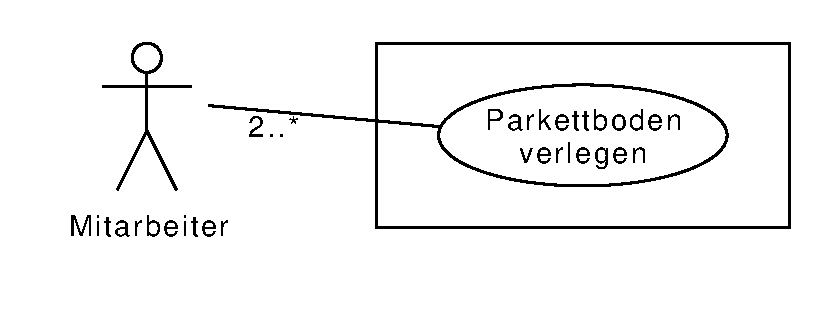
\includegraphics[scale=0.5]{Aufgabe4c.pdf}
        \end{center}
    \end{enumerate}
  \end{solution}
  
\newpage
  
  \problemnumber{5}
  \begin{problem}
    
  \end{problem}
  \begin{solution}\hfill
    \begin{center}
      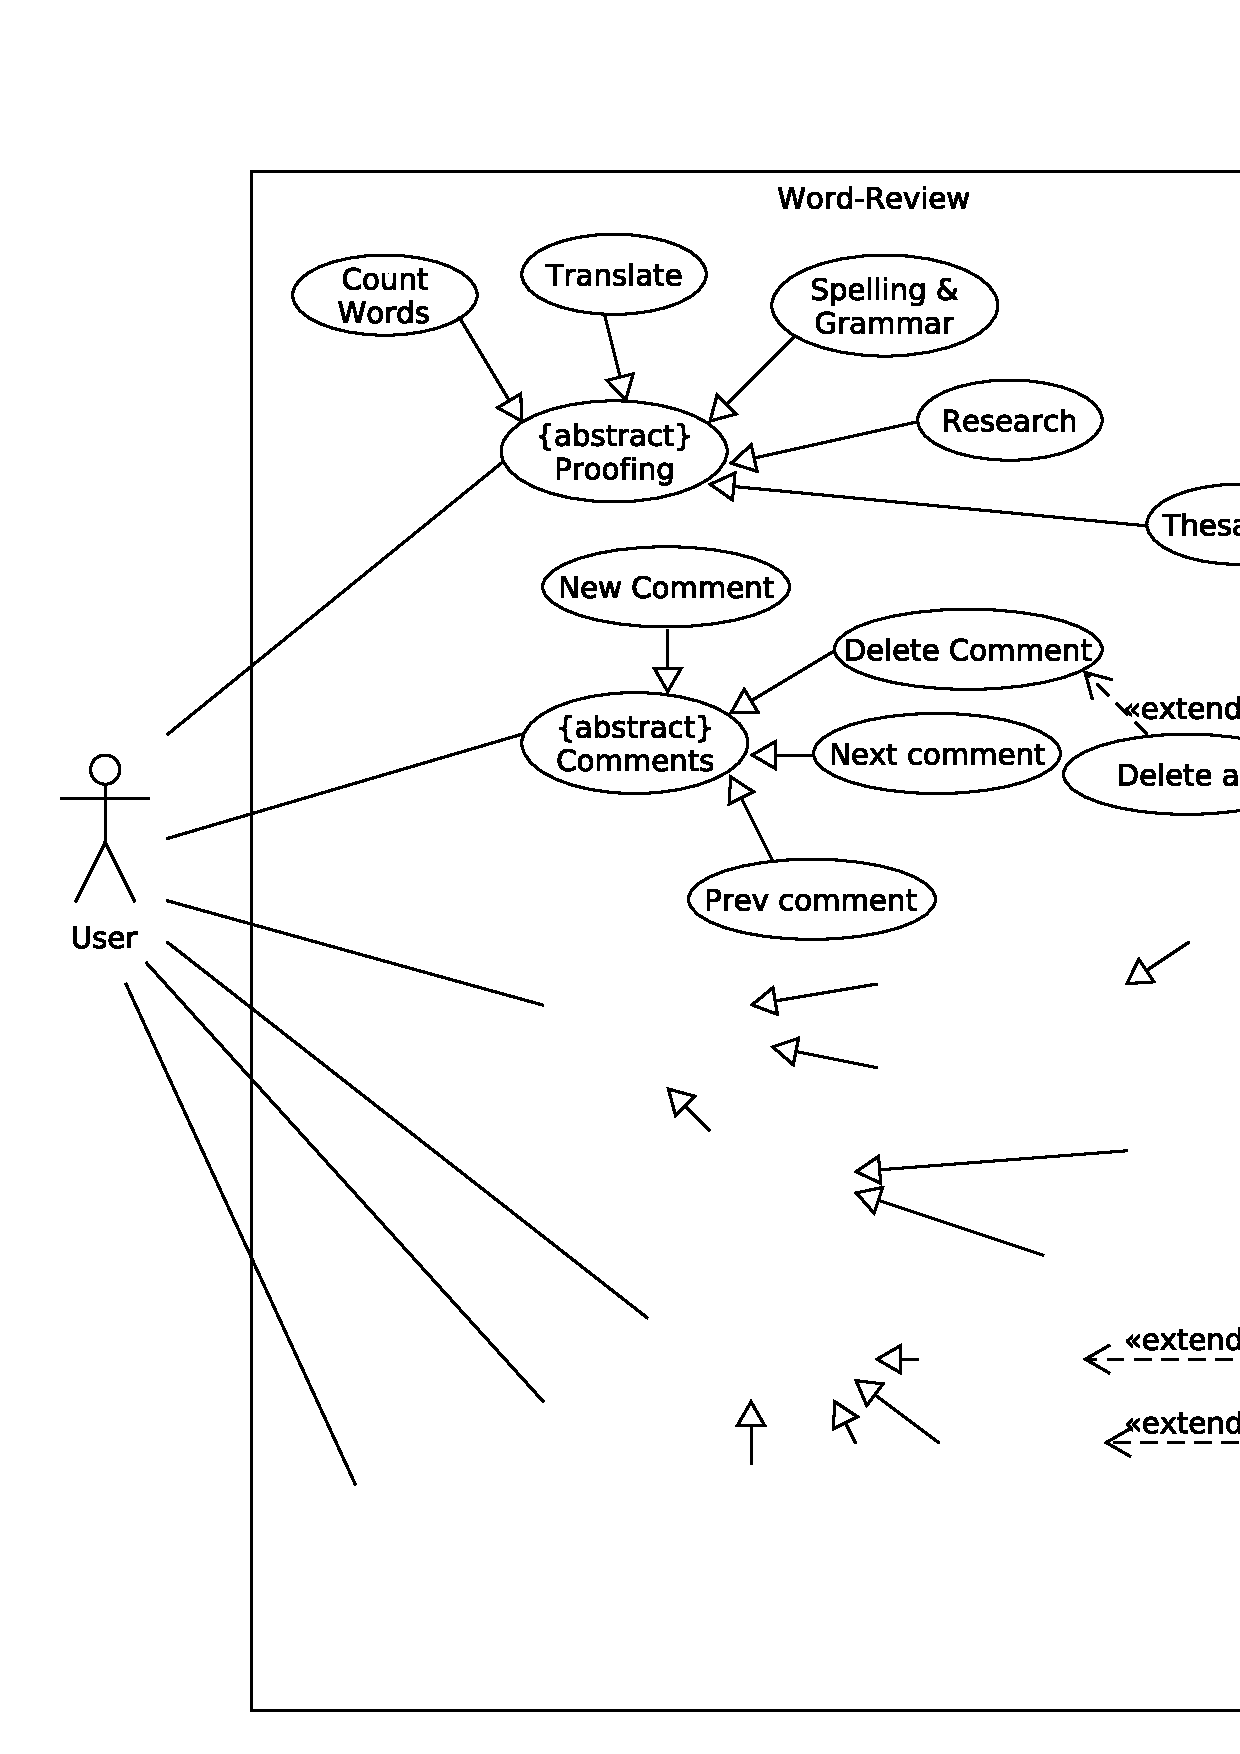
\includegraphics[scale=0.6]{Aufgabe5.pdf}
    \end{center}
  \end{solution}



\end{document}